\tikzset{every picture/.style={line width=0.75pt}} %set default line width to 0.75pt        

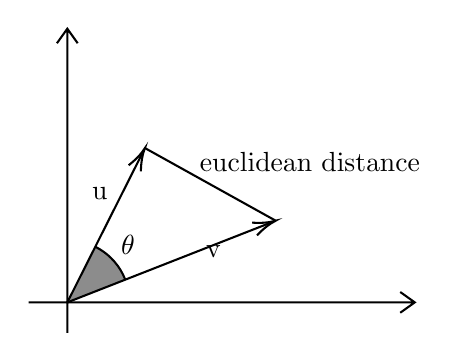
\begin{tikzpicture}[x=0.75pt,y=0.75pt,yscale=-1,xscale=1]
%uncomment if require: \path (0,300); %set diagram left start at 0, and has height of 300

%Shape: Axis 2D [id:dp9247573707891508] 
\draw  (50,199.85) -- (236,199.85)(68.6,68) -- (68.6,214.5) (229,194.85) -- (236,199.85) -- (229,204.85) (63.6,75) -- (68.6,68) -- (73.6,75)  ;
%Straight Lines [id:da4418715205409134] 
\draw    (68.6,199.85) -- (167.14,161.23) ;
\draw [shift={(169,160.5)}, rotate = 158.6] [color={rgb, 255:red, 0; green, 0; blue, 0 }  ][line width=0.75]    (10.93,-3.29) .. controls (6.95,-1.4) and (3.31,-0.3) .. (0,0) .. controls (3.31,0.3) and (6.95,1.4) .. (10.93,3.29)   ;
%Straight Lines [id:da9719047623164807] 
\draw    (68.6,199.85) -- (95.55,146.27) -- (105.1,127.29) ;
\draw [shift={(106,125.5)}, rotate = 116.7] [color={rgb, 255:red, 0; green, 0; blue, 0 }  ][line width=0.75]    (10.93,-3.29) .. controls (6.95,-1.4) and (3.31,-0.3) .. (0,0) .. controls (3.31,0.3) and (6.95,1.4) .. (10.93,3.29)   ;
%Shape: Arc [id:dp7509394088510173] 
\draw  [draw opacity=0][fill={rgb, 255:red, 0; green, 0; blue, 0 }  ,fill opacity=0.45 ] (82.33,173.17) .. controls (87.77,175.97) and (92.42,180.45) .. (95.38,186.34) .. controls (95.78,187.12) and (96.14,187.92) .. (96.46,188.72) -- (68.6,199.85) -- cycle ; \draw   (82.33,173.17) .. controls (87.77,175.97) and (92.42,180.45) .. (95.38,186.34) .. controls (95.78,187.12) and (96.14,187.92) .. (96.46,188.72) ;  
%Straight Lines [id:da2404981848512595] 
\draw    (106,125.5) -- (169,160.5) ;

% Text Node
\draw (93,166) node [anchor=north west][inner sep=0.75pt]   [align=left] {$\displaystyle \theta $};
% Text Node
\draw (131,126) node [anchor=north west][inner sep=0.75pt]   [align=left] {euclidean distance};
% Text Node
\draw (79,143) node [anchor=north west][inner sep=0.75pt]   [align=left] {u};
% Text Node
\draw (134,171) node [anchor=north west][inner sep=0.75pt]   [align=left] {v};


\end{tikzpicture}